% Options for packages loaded elsewhere
\PassOptionsToPackage{unicode}{hyperref}
\PassOptionsToPackage{hyphens}{url}
%
\documentclass[
]{article}
\usepackage{lmodern}
\usepackage{amssymb,amsmath}
\usepackage{ifxetex,ifluatex}
\ifnum 0\ifxetex 1\fi\ifluatex 1\fi=0 % if pdftex
  \usepackage[T1]{fontenc}
  \usepackage[utf8]{inputenc}
  \usepackage{textcomp} % provide euro and other symbols
\else % if luatex or xetex
  \usepackage{unicode-math}
  \defaultfontfeatures{Scale=MatchLowercase}
  \defaultfontfeatures[\rmfamily]{Ligatures=TeX,Scale=1}
\fi
% Use upquote if available, for straight quotes in verbatim environments
\IfFileExists{upquote.sty}{\usepackage{upquote}}{}
\IfFileExists{microtype.sty}{% use microtype if available
  \usepackage[]{microtype}
  \UseMicrotypeSet[protrusion]{basicmath} % disable protrusion for tt fonts
}{}
\makeatletter
\@ifundefined{KOMAClassName}{% if non-KOMA class
  \IfFileExists{parskip.sty}{%
    \usepackage{parskip}
  }{% else
    \setlength{\parindent}{0pt}
    \setlength{\parskip}{6pt plus 2pt minus 1pt}}
}{% if KOMA class
  \KOMAoptions{parskip=half}}
\makeatother
\usepackage{xcolor}
\IfFileExists{xurl.sty}{\usepackage{xurl}}{} % add URL line breaks if available
\IfFileExists{bookmark.sty}{\usepackage{bookmark}}{\usepackage{hyperref}}
\hypersetup{
  pdftitle={Seshat},
  pdfauthor={Achille-Laurent},
  hidelinks,
  pdfcreator={LaTeX via pandoc}}
\urlstyle{same} % disable monospaced font for URLs
\usepackage[margin=1in]{geometry}
\usepackage{color}
\usepackage{fancyvrb}
\newcommand{\VerbBar}{|}
\newcommand{\VERB}{\Verb[commandchars=\\\{\}]}
\DefineVerbatimEnvironment{Highlighting}{Verbatim}{commandchars=\\\{\}}
% Add ',fontsize=\small' for more characters per line
\usepackage{framed}
\definecolor{shadecolor}{RGB}{248,248,248}
\newenvironment{Shaded}{\begin{snugshade}}{\end{snugshade}}
\newcommand{\AlertTok}[1]{\textcolor[rgb]{0.94,0.16,0.16}{#1}}
\newcommand{\AnnotationTok}[1]{\textcolor[rgb]{0.56,0.35,0.01}{\textbf{\textit{#1}}}}
\newcommand{\AttributeTok}[1]{\textcolor[rgb]{0.77,0.63,0.00}{#1}}
\newcommand{\BaseNTok}[1]{\textcolor[rgb]{0.00,0.00,0.81}{#1}}
\newcommand{\BuiltInTok}[1]{#1}
\newcommand{\CharTok}[1]{\textcolor[rgb]{0.31,0.60,0.02}{#1}}
\newcommand{\CommentTok}[1]{\textcolor[rgb]{0.56,0.35,0.01}{\textit{#1}}}
\newcommand{\CommentVarTok}[1]{\textcolor[rgb]{0.56,0.35,0.01}{\textbf{\textit{#1}}}}
\newcommand{\ConstantTok}[1]{\textcolor[rgb]{0.00,0.00,0.00}{#1}}
\newcommand{\ControlFlowTok}[1]{\textcolor[rgb]{0.13,0.29,0.53}{\textbf{#1}}}
\newcommand{\DataTypeTok}[1]{\textcolor[rgb]{0.13,0.29,0.53}{#1}}
\newcommand{\DecValTok}[1]{\textcolor[rgb]{0.00,0.00,0.81}{#1}}
\newcommand{\DocumentationTok}[1]{\textcolor[rgb]{0.56,0.35,0.01}{\textbf{\textit{#1}}}}
\newcommand{\ErrorTok}[1]{\textcolor[rgb]{0.64,0.00,0.00}{\textbf{#1}}}
\newcommand{\ExtensionTok}[1]{#1}
\newcommand{\FloatTok}[1]{\textcolor[rgb]{0.00,0.00,0.81}{#1}}
\newcommand{\FunctionTok}[1]{\textcolor[rgb]{0.00,0.00,0.00}{#1}}
\newcommand{\ImportTok}[1]{#1}
\newcommand{\InformationTok}[1]{\textcolor[rgb]{0.56,0.35,0.01}{\textbf{\textit{#1}}}}
\newcommand{\KeywordTok}[1]{\textcolor[rgb]{0.13,0.29,0.53}{\textbf{#1}}}
\newcommand{\NormalTok}[1]{#1}
\newcommand{\OperatorTok}[1]{\textcolor[rgb]{0.81,0.36,0.00}{\textbf{#1}}}
\newcommand{\OtherTok}[1]{\textcolor[rgb]{0.56,0.35,0.01}{#1}}
\newcommand{\PreprocessorTok}[1]{\textcolor[rgb]{0.56,0.35,0.01}{\textit{#1}}}
\newcommand{\RegionMarkerTok}[1]{#1}
\newcommand{\SpecialCharTok}[1]{\textcolor[rgb]{0.00,0.00,0.00}{#1}}
\newcommand{\SpecialStringTok}[1]{\textcolor[rgb]{0.31,0.60,0.02}{#1}}
\newcommand{\StringTok}[1]{\textcolor[rgb]{0.31,0.60,0.02}{#1}}
\newcommand{\VariableTok}[1]{\textcolor[rgb]{0.00,0.00,0.00}{#1}}
\newcommand{\VerbatimStringTok}[1]{\textcolor[rgb]{0.31,0.60,0.02}{#1}}
\newcommand{\WarningTok}[1]{\textcolor[rgb]{0.56,0.35,0.01}{\textbf{\textit{#1}}}}
\usepackage{graphicx,grffile}
\makeatletter
\def\maxwidth{\ifdim\Gin@nat@width>\linewidth\linewidth\else\Gin@nat@width\fi}
\def\maxheight{\ifdim\Gin@nat@height>\textheight\textheight\else\Gin@nat@height\fi}
\makeatother
% Scale images if necessary, so that they will not overflow the page
% margins by default, and it is still possible to overwrite the defaults
% using explicit options in \includegraphics[width, height, ...]{}
\setkeys{Gin}{width=\maxwidth,height=\maxheight,keepaspectratio}
% Set default figure placement to htbp
\makeatletter
\def\fps@figure{htbp}
\makeatother
\setlength{\emergencystretch}{3em} % prevent overfull lines
\providecommand{\tightlist}{%
  \setlength{\itemsep}{0pt}\setlength{\parskip}{0pt}}
\setcounter{secnumdepth}{-\maxdimen} % remove section numbering

\title{Seshat}
\author{Achille-Laurent}
\date{03/06/2020}

\begin{document}
\maketitle

\hypertarget{analyse-de-la-base-seshat}{%
\section{Analyse de la base Seshat}\label{analyse-de-la-base-seshat}}

Code concernant la première approche, l'ACP, la classification et la
régression

\hypertarget{donnuxe9es-axial}{%
\section{1. Données Axial}\label{donnuxe9es-axial}}

\hypertarget{importation}{%
\subsection{1.1 Importation}\label{importation}}

\begin{Shaded}
\begin{Highlighting}[]
\NormalTok{dfn <-}\StringTok{ }\KeywordTok{read.csv}\NormalTok{(}\StringTok{'../databases/axial_index.csv'}\NormalTok{,}\DataTypeTok{sep=}\StringTok{','}\NormalTok{)}
\CommentTok{# Mettre l'Index en index et retirer SPC1}
\NormalTok{data <-}\StringTok{ }\KeywordTok{subset}\NormalTok{(dfn, }\DataTypeTok{select=}\OperatorTok{-}\KeywordTok{c}\NormalTok{(Index,Time,NGA,PolID))}
\KeywordTok{rownames}\NormalTok{(data) <-}\StringTok{ }\NormalTok{dfn}\OperatorTok{$}\NormalTok{Index}
\KeywordTok{attach}\NormalTok{(data)}
\KeywordTok{head}\NormalTok{(data)}
\end{Highlighting}
\end{Shaded}

\begin{verbatim}
##                       PolPop  PolTerr   CapPop      levels government infrastr
## Konya Plain (-9600) 3.293724 4.138263 1.442118 -0.05581711          0        0
## Konya Plain (-9500) 3.293724 4.138263 1.442118 -0.05581711          0        0
## Konya Plain (-9400) 3.293724 4.138263 1.442118 -0.05581711          0        0
## Konya Plain (-9300) 3.293724 4.138263 1.442118 -0.05581711          0        0
## Konya Plain (-9200) 3.293724 4.138263 1.442118 -0.05581711          0        0
## Konya Plain (-9100) 3.293724 4.138263 1.442118 -0.05581711          0        0
##                     writing texts money
## Konya Plain (-9600)       0     0     0
## Konya Plain (-9500)       0     0     0
## Konya Plain (-9400)       0     0     0
## Konya Plain (-9300)       0     0     0
## Konya Plain (-9200)       0     0     0
## Konya Plain (-9100)       0     0     0
\end{verbatim}

\hypertarget{vue-densemble}{%
\subsection{1.2. Vue d'ensemble}\label{vue-densemble}}

\begin{Shaded}
\begin{Highlighting}[]
\CommentTok{# Séparer les 2 plots qui sont d'échelle différente}
\KeywordTok{boxplot}\NormalTok{(}\KeywordTok{subset}\NormalTok{(data,}\DataTypeTok{select =} \KeywordTok{c}\NormalTok{(PolPop,PolTerr,CapPop,levels,money)))}
\end{Highlighting}
\end{Shaded}

\includegraphics{seshat_achille_files/figure-latex/unnamed-chunk-2-1.pdf}

\begin{Shaded}
\begin{Highlighting}[]
\KeywordTok{boxplot}\NormalTok{(}\KeywordTok{subset}\NormalTok{(data,}\DataTypeTok{select =} \KeywordTok{c}\NormalTok{(government,infrastr,writing,texts)))}
\end{Highlighting}
\end{Shaded}

\includegraphics{seshat_achille_files/figure-latex/unnamed-chunk-2-2.pdf}

\hypertarget{analyse-en-composante-principale}{%
\section{2. Analyse en Composante
Principale}\label{analyse-en-composante-principale}}

\begin{Shaded}
\begin{Highlighting}[]
\NormalTok{X=}\StringTok{ }\KeywordTok{scale}\NormalTok{(data, }\DataTypeTok{center=}\NormalTok{T, }\DataTypeTok{scale=}\NormalTok{T) }

\NormalTok{S =}\StringTok{ }\KeywordTok{cov}\NormalTok{(X)}
\NormalTok{acp =}\StringTok{ }\KeywordTok{eigen}\NormalTok{(S)}
\NormalTok{lambda =}\StringTok{ }\NormalTok{acp}\OperatorTok{$}\NormalTok{values}
\NormalTok{vecteurs_propres =}\StringTok{ }\NormalTok{acp}\OperatorTok{$}\NormalTok{vectors}
\NormalTok{Inertie =}\StringTok{ }\KeywordTok{sum}\NormalTok{(}\KeywordTok{diag}\NormalTok{(S))}
\NormalTok{part.inertie =}\StringTok{ }\NormalTok{lambda}\OperatorTok{/}\KeywordTok{sum}\NormalTok{(lambda)}
\end{Highlighting}
\end{Shaded}

\hypertarget{explication}{%
\subsection{2.1 Explication}\label{explication}}

\begin{Shaded}
\begin{Highlighting}[]
\KeywordTok{barplot}\NormalTok{(lambda}\OperatorTok{/}\KeywordTok{sum}\NormalTok{(lambda),}\DataTypeTok{names.arg =} \DecValTok{1}\OperatorTok{:}\KeywordTok{length}\NormalTok{(lambda))}
\KeywordTok{title}\NormalTok{(}\DataTypeTok{main=}\StringTok{"Explication des différentes composantes"}\NormalTok{)}
\end{Highlighting}
\end{Shaded}

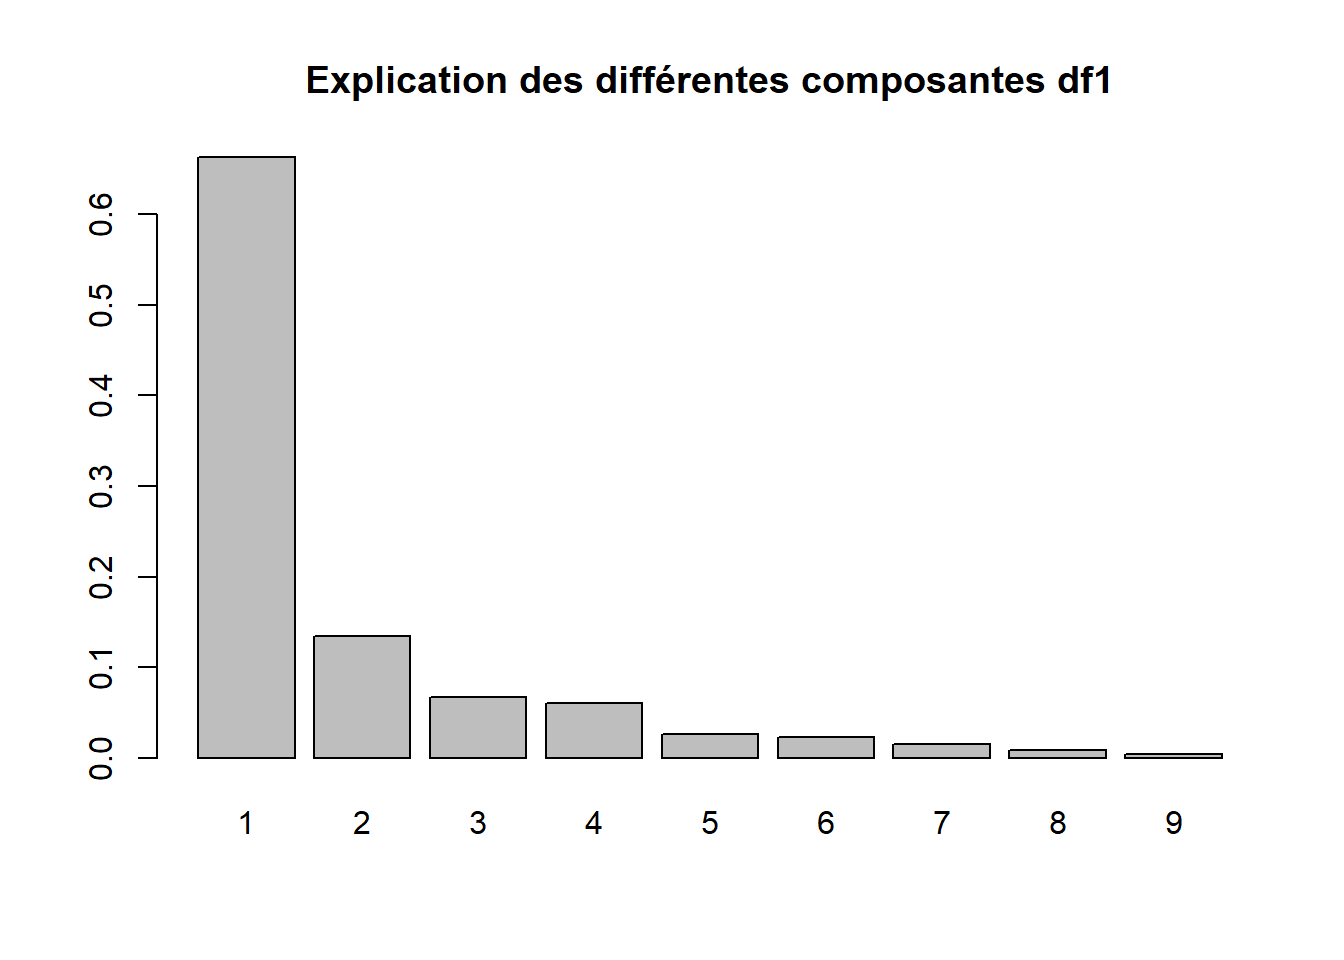
\includegraphics{seshat_achille_files/figure-latex/unnamed-chunk-4-1.pdf}
\#\# 2.2. Projection

\begin{Shaded}
\begin{Highlighting}[]
\CommentTok{# Les composantes principales : }
\NormalTok{C =}\StringTok{ }\NormalTok{X }\OperatorTok\StringTok{ }\NormalTok{vecteurs_propres}
\CommentTok{# colnames(C) =   paste("comp", 1:4)}
\KeywordTok{plot}\NormalTok{(C[,}\DecValTok{1}\OperatorTok{:}\DecValTok{2}\NormalTok{],}\DataTypeTok{type=}\StringTok{"p"}\NormalTok{,}\DataTypeTok{xlab=}\StringTok{'PC1'}\NormalTok{,}\DataTypeTok{ylab=}\StringTok{'PC2'}\NormalTok{)}
\CommentTok{# text(C[,1:2])}
\KeywordTok{title}\NormalTok{(}\DataTypeTok{main=}\StringTok{"Projection sur les 2 premiers axes principaux"}\NormalTok{)}
\KeywordTok{lines}\NormalTok{(}\KeywordTok{c}\NormalTok{(}\KeywordTok{min}\NormalTok{(C[,}\DecValTok{1}\NormalTok{]),}\KeywordTok{max}\NormalTok{(C[,}\DecValTok{1}\NormalTok{])),}\KeywordTok{c}\NormalTok{(}\DecValTok{0}\NormalTok{,}\DecValTok{0}\NormalTok{))}
\KeywordTok{lines}\NormalTok{(}\KeywordTok{c}\NormalTok{(}\DecValTok{0}\NormalTok{,}\DecValTok{0}\NormalTok{),}\KeywordTok{c}\NormalTok{(}\KeywordTok{min}\NormalTok{(C[,}\DecValTok{2}\NormalTok{]),}\KeywordTok{max}\NormalTok{(C[,}\DecValTok{2}\NormalTok{])))}
\end{Highlighting}
\end{Shaded}

\includegraphics{seshat_achille_files/figure-latex/unnamed-chunk-5-1.pdf}
\#\# 2.3 Composantes principales PC1 et PC2

\begin{Shaded}
\begin{Highlighting}[]
\KeywordTok{barplot}\NormalTok{(}\OperatorTok{-}\NormalTok{vecteurs_propres[,}\DecValTok{1}\NormalTok{],}\DataTypeTok{ylab =} \StringTok{'Contribution'}\NormalTok{,}\DataTypeTok{xlab =} \StringTok{'Variables'}\NormalTok{,}\DataTypeTok{names.arg =} \KeywordTok{names}\NormalTok{(data),}\DataTypeTok{axes =} \OtherTok{TRUE}\NormalTok{)}
\KeywordTok{title}\NormalTok{(}\DataTypeTok{main=}\StringTok{"Contributions des variables au PC1"}\NormalTok{)}
\end{Highlighting}
\end{Shaded}

\includegraphics{seshat_achille_files/figure-latex/unnamed-chunk-6-1.pdf}

\begin{Shaded}
\begin{Highlighting}[]
\KeywordTok{barplot}\NormalTok{(}\OperatorTok{-}\NormalTok{vecteurs_propres[,}\DecValTok{2}\NormalTok{],}\DataTypeTok{ylab =} \StringTok{'Contribution'}\NormalTok{,}\DataTypeTok{xlab =} \StringTok{'Variables'}\NormalTok{,}\DataTypeTok{names.arg =} \KeywordTok{names}\NormalTok{(data),}\DataTypeTok{axes =} \OtherTok{TRUE}\NormalTok{)}
\KeywordTok{title}\NormalTok{(}\DataTypeTok{main=}\StringTok{"Contributions des variables au PC2"}\NormalTok{)}
\end{Highlighting}
\end{Shaded}

\includegraphics{seshat_achille_files/figure-latex/unnamed-chunk-6-2.pdf}

\hypertarget{avec-factominer}{%
\subsection{2.4 Avec FactoMineR}\label{avec-factominer}}

\begin{Shaded}
\begin{Highlighting}[]
\KeywordTok{library}\NormalTok{(FactoMineR)}
\NormalTok{pca <-}\StringTok{ }\KeywordTok{PCA}\NormalTok{(data, }\DataTypeTok{scale.unit =} \OtherTok{TRUE}\NormalTok{, }\DataTypeTok{ncp =} \DecValTok{11}\NormalTok{, }\DataTypeTok{graph =} \OtherTok{TRUE}\NormalTok{)}
\end{Highlighting}
\end{Shaded}

\includegraphics{seshat_achille_files/figure-latex/unnamed-chunk-7-1.pdf}
\includegraphics{seshat_achille_files/figure-latex/unnamed-chunk-7-2.pdf}

\hypertarget{k-means}{%
\section{3 k-means}\label{k-means}}

On a vu sur l'ACP qu'on pouvait distinguer environ deux groupes. On
essaie des k-means :

\hypertarget{projection}{%
\subsection{3.1 Projection}\label{projection}}

\begin{Shaded}
\begin{Highlighting}[]
\NormalTok{kmeans.result =}\StringTok{ }\KeywordTok{kmeans}\NormalTok{(data,}\DecValTok{3}\NormalTok{)}
\KeywordTok{plot}\NormalTok{(C[,}\DecValTok{1}\OperatorTok{:}\DecValTok{2}\NormalTok{],}\DataTypeTok{type=}\StringTok{"p"}\NormalTok{,}\DataTypeTok{xlab=}\StringTok{'PC1'}\NormalTok{,}\DataTypeTok{ylab=}\StringTok{'PC2'}\NormalTok{,}\DataTypeTok{col =}\NormalTok{ kmeans.result}\OperatorTok{$}\NormalTok{cluster}\OperatorTok{+}\DecValTok{3}\NormalTok{)}
\end{Highlighting}
\end{Shaded}

\includegraphics{seshat_achille_files/figure-latex/unnamed-chunk-8-1.pdf}

\begin{Shaded}
\begin{Highlighting}[]
\NormalTok{kmeans.result =}\StringTok{ }\KeywordTok{kmeans}\NormalTok{(data,}\DecValTok{2}\NormalTok{)}
\KeywordTok{plot}\NormalTok{(C[,}\DecValTok{1}\OperatorTok{:}\DecValTok{2}\NormalTok{],}\DataTypeTok{type=}\StringTok{"p"}\NormalTok{,}\DataTypeTok{xlab=}\StringTok{'PC1'}\NormalTok{,}\DataTypeTok{ylab=}\StringTok{'PC2'}\NormalTok{,}\DataTypeTok{col =}\NormalTok{kmeans.result}\OperatorTok{$}\NormalTok{cluster)}
\end{Highlighting}
\end{Shaded}

\includegraphics{seshat_achille_files/figure-latex/unnamed-chunk-8-2.pdf}

Pour k = 3, on a un groupe qui contient les points dispersés du milieu.
\#\# 3.2 CAH Pour savoir quelle classification est la plus pertinente,
essayons un CAH :

\begin{Shaded}
\begin{Highlighting}[]
\NormalTok{hc <-}\StringTok{ }\KeywordTok{hclust}\NormalTok{(}\KeywordTok{dist}\NormalTok{(data))}
\KeywordTok{plot}\NormalTok{(hc,}\DataTypeTok{hang=}\OperatorTok{-}\DecValTok{1}\NormalTok{,}\DataTypeTok{labels =} \OtherTok{FALSE}\NormalTok{)}
\KeywordTok{rect.hclust}\NormalTok{(hc,}\DataTypeTok{k=}\DecValTok{2}\NormalTok{,}\DataTypeTok{border =} \DecValTok{4}\NormalTok{)}
\KeywordTok{rect.hclust}\NormalTok{(hc,}\DataTypeTok{k=}\DecValTok{3}\NormalTok{)}
\end{Highlighting}
\end{Shaded}

\includegraphics{seshat_achille_files/figure-latex/unnamed-chunk-9-1.pdf}

\begin{Shaded}
\begin{Highlighting}[]
\KeywordTok{barplot}\NormalTok{(hc}\OperatorTok{$}\NormalTok{height[(}\KeywordTok{length}\NormalTok{(hc}\OperatorTok{$}\NormalTok{height)}\OperatorTok{-}\DecValTok{10}\NormalTok{)}\OperatorTok{:}\NormalTok{(}\KeywordTok{length}\NormalTok{(hc}\OperatorTok{$}\NormalTok{height))])}
\end{Highlighting}
\end{Shaded}

\includegraphics{seshat_achille_files/figure-latex/unnamed-chunk-9-2.pdf}

\hypertarget{comparaisons-des-deux-clusters}{%
\subsection{3.3 Comparaisons des deux
clusters}\label{comparaisons-des-deux-clusters}}

Une fois les groupes réunis, il serait intéressant de comprendre ce qui
les distingue, les deux dimensions n'y suffisent pas entièrement :

\begin{Shaded}
\begin{Highlighting}[]
\CommentTok{# Kmeans pour k choisi}
\NormalTok{k =}\StringTok{ }\DecValTok{2} 
\NormalTok{kmeans.result =}\StringTok{ }\KeywordTok{kmeans}\NormalTok{(data,k)}
\KeywordTok{plot}\NormalTok{(C[,}\DecValTok{1}\OperatorTok{:}\DecValTok{2}\NormalTok{],}\DataTypeTok{type=}\StringTok{"p"}\NormalTok{,}\DataTypeTok{xlab=}\StringTok{'PC1'}\NormalTok{,}\DataTypeTok{ylab=}\StringTok{'PC2'}\NormalTok{,}\DataTypeTok{col =}\NormalTok{ kmeans.result}\OperatorTok{$}\NormalTok{cluster)}
\end{Highlighting}
\end{Shaded}

\includegraphics{seshat_achille_files/figure-latex/unnamed-chunk-10-1.pdf}

\begin{Shaded}
\begin{Highlighting}[]
\CommentTok{# Affichage des grandes variables}
\NormalTok{data.grand =}\StringTok{ }\KeywordTok{subset}\NormalTok{(data,}\DataTypeTok{select =} \KeywordTok{c}\NormalTok{(PolPop,PolTerr,CapPop,levels,money))}
\NormalTok{data.grand.all =}\StringTok{ }\KeywordTok{list}\NormalTok{()}
\ControlFlowTok{for}\NormalTok{(nom }\ControlFlowTok{in} \KeywordTok{names}\NormalTok{(data.grand))}
\NormalTok{\{}
  \ControlFlowTok{for}\NormalTok{(i }\ControlFlowTok{in} \DecValTok{1}\OperatorTok{:}\NormalTok{k)}
\NormalTok{  \{}
\NormalTok{      data.grand.all[[}\KeywordTok{paste}\NormalTok{(nom,i)]] <-}\StringTok{ }\NormalTok{data.grand[kmeans.result}\OperatorTok{$}\NormalTok{cluster}\OperatorTok{==}\NormalTok{i,nom]}
\NormalTok{  \}}
\NormalTok{\}}
\KeywordTok{boxplot}\NormalTok{(data.grand.all,}\DataTypeTok{col =} \KeywordTok{rep}\NormalTok{(}\KeywordTok{c}\NormalTok{(}\DecValTok{2}\OperatorTok{:}\NormalTok{(k}\OperatorTok{+}\DecValTok{1}\NormalTok{)),}\KeywordTok{length}\NormalTok{(data.grand)))}
\end{Highlighting}
\end{Shaded}

\includegraphics{seshat_achille_files/figure-latex/unnamed-chunk-10-2.pdf}

\begin{Shaded}
\begin{Highlighting}[]
\CommentTok{# Affichage des petites variables}
\NormalTok{data.petit =}\StringTok{ }\KeywordTok{subset}\NormalTok{(data,}\DataTypeTok{select =} \KeywordTok{c}\NormalTok{(government,infrastr,writing,texts))}
\NormalTok{data.petit.all =}\StringTok{ }\KeywordTok{list}\NormalTok{()}
\ControlFlowTok{for}\NormalTok{(nom }\ControlFlowTok{in} \KeywordTok{names}\NormalTok{(data.petit))}
\NormalTok{\{}
  \ControlFlowTok{for}\NormalTok{(i }\ControlFlowTok{in} \DecValTok{1}\OperatorTok{:}\NormalTok{k)}
\NormalTok{  \{}
\NormalTok{      data.petit.all[[}\KeywordTok{paste}\NormalTok{(nom,i)]] <-}\StringTok{ }\NormalTok{data.petit[kmeans.result}\OperatorTok{$}\NormalTok{cluster}\OperatorTok{==}\NormalTok{i,nom]}
\NormalTok{  \}}
\NormalTok{\}}
\KeywordTok{boxplot}\NormalTok{(data.petit.all,}\DataTypeTok{col =} \KeywordTok{rep}\NormalTok{(}\KeywordTok{c}\NormalTok{(}\DecValTok{2}\OperatorTok{:}\NormalTok{(k}\OperatorTok{+}\DecValTok{1}\NormalTok{)),}\KeywordTok{length}\NormalTok{(data.petit)))}
\end{Highlighting}
\end{Shaded}

\includegraphics{seshat_achille_files/figure-latex/unnamed-chunk-10-3.pdf}

\hypertarget{analyse-sur-la-base-morale}{%
\section{4. Analyse sur la base
Morale}\label{analyse-sur-la-base-morale}}

On utilise les nouveaux groupes ppur tenter de classifier avec des
forêts sur les variables morales

\begin{Shaded}
\begin{Highlighting}[]
\KeywordTok{detach}\NormalTok{(data)}
\end{Highlighting}
\end{Shaded}

\hypertarget{cruxe9ation-des-donnuxe9es}{%
\subsection{4.1 Création des données}\label{cruxe9ation-des-donnuxe9es}}

\begin{Shaded}
\begin{Highlighting}[]
\NormalTok{dfm <-}\StringTok{ }\KeywordTok{read.csv}\NormalTok{(}\StringTok{'../databases/morale_index_inaxe.csv'}\NormalTok{,}\DataTypeTok{sep=}\StringTok{','}\NormalTok{)}

\CommentTok{# Mettre l'Index en index et retirer SPC1}
\NormalTok{datam <-}\StringTok{ }\KeywordTok{subset}\NormalTok{(dfm, }\DataTypeTok{select=}\OperatorTok{-}\KeywordTok{c}\NormalTok{(Index,Time,NGA,sum))}
\KeywordTok{rownames}\NormalTok{(datam) <-}\StringTok{ }\NormalTok{dfm}\OperatorTok{$}\NormalTok{Index}
\KeywordTok{attach}\NormalTok{(datam)}

\CommentTok{# On associe ensuite à chaque individu dans la base morale son cluster (1 ou 2) correspondant}
\NormalTok{rreess <-}\StringTok{ }\NormalTok{kmeans.result}\OperatorTok{$}\NormalTok{cluster}
\NormalTok{datam}\OperatorTok{$}\NormalTok{cluster <-}\StringTok{ }\NormalTok{(rreess[(dfn}\OperatorTok{$}\NormalTok{Index)}\OperatorTok\NormalTok{(dfm}\OperatorTok{$}\NormalTok{Index)] }\OperatorTok{==}\DecValTok{1}\NormalTok{)}\OperatorTok{*}\DecValTok{1}

\KeywordTok{head}\NormalTok{(datam)}
\end{Highlighting}
\end{Shaded}

\begin{verbatim}
##                     X1._Moralistic_punishment X2._Moralizing_norms
## Upper Egypt (-4400)                         0                    0
## Upper Egypt (-4300)                         0                    0
## Upper Egypt (-4200)                         0                    0
## Upper Egypt (-4100)                         0                    0
## Upper Egypt (-4000)                         0                    0
## Upper Egypt (-3900)                         0                    0
##                     X3._Promotion_of_prosociality
## Upper Egypt (-4400)                             0
## Upper Egypt (-4300)                             0
## Upper Egypt (-4200)                             0
## Upper Egypt (-4100)                             0
## Upper Egypt (-4000)                             0
## Upper Egypt (-3900)                             0
##                     X4._Omniscient_supernatural_beings X5._Rulers_not_gods
## Upper Egypt (-4400)                                  0                   0
## Upper Egypt (-4300)                                  0                   0
## Upper Egypt (-4200)                                  0                   0
## Upper Egypt (-4100)                                  0                   0
## Upper Egypt (-4000)                                  0                   0
## Upper Egypt (-3900)                                  0                   0
##                     X6._Equating_elites_and_commoners
## Upper Egypt (-4400)                                 0
## Upper Egypt (-4300)                                 0
## Upper Egypt (-4200)                                 0
## Upper Egypt (-4100)                                 0
## Upper Egypt (-4000)                                 0
## Upper Egypt (-3900)                                 0
##                     X7._Equating_rulers_and_commoners X8._Formal_legal_code
## Upper Egypt (-4400)                                 0                     0
## Upper Egypt (-4300)                                 0                     0
## Upper Egypt (-4200)                                 0                     0
## Upper Egypt (-4100)                                 0                     0
## Upper Egypt (-4000)                                 0                     0
## Upper Egypt (-3900)                                 0                     0
##                     X9._General_applicability_of_law
## Upper Egypt (-4400)                                0
## Upper Egypt (-4300)                                0
## Upper Egypt (-4200)                                0
## Upper Egypt (-4100)                                0
## Upper Egypt (-4000)                                0
## Upper Egypt (-3900)                                0
##                     X10._Constraint_on_executive X11._Full.time_bureaucrats
## Upper Egypt (-4400)                            0                          0
## Upper Egypt (-4300)                            0                          0
## Upper Egypt (-4200)                            0                          0
## Upper Egypt (-4100)                            0                          0
## Upper Egypt (-4000)                            0                          0
## Upper Egypt (-3900)                            0                          0
##                     X12._Impeachment cluster
## Upper Egypt (-4400)                0       1
## Upper Egypt (-4300)                0       1
## Upper Egypt (-4200)                0       1
## Upper Egypt (-4100)                0       1
## Upper Egypt (-4000)                0       1
## Upper Egypt (-3900)                0       1
\end{verbatim}

\hypertarget{arbre}{%
\subsection{4.2 Arbre}\label{arbre}}

\begin{Shaded}
\begin{Highlighting}[]
\KeywordTok{library}\NormalTok{(rpart)}
\NormalTok{arbre=}\KeywordTok{rpart}\NormalTok{(datam}\OperatorTok{$}\NormalTok{cluster}\OperatorTok{~}\NormalTok{.,datam)}
\CommentTok{# summary(arbre)}
\CommentTok{# print(arbre)}
\KeywordTok{library}\NormalTok{(rpart.plot)}
\KeywordTok{rpart.plot}\NormalTok{(arbre, }\DataTypeTok{type=}\DecValTok{4}\NormalTok{, }\DataTypeTok{digits=}\DecValTok{3}\NormalTok{)}
\end{Highlighting}
\end{Shaded}

\includegraphics{seshat_achille_files/figure-latex/unnamed-chunk-13-1.pdf}
\#\# 4.3 Régression \#\# 4.3.1 Modèle

\begin{Shaded}
\begin{Highlighting}[]
\NormalTok{res <-}\StringTok{ }\KeywordTok{glm}\NormalTok{(cluster}\OperatorTok{~}\NormalTok{.,}\DataTypeTok{family=}\NormalTok{binomial,}\DataTypeTok{data=}\NormalTok{datam)}
\KeywordTok{summary}\NormalTok{(res)}
\end{Highlighting}
\end{Shaded}

\begin{verbatim}
## 
## Call:
## glm(formula = cluster ~ ., family = binomial, data = datam)
## 
## Deviance Residuals: 
##     Min       1Q   Median       3Q      Max  
## -1.6117  -0.5118  -0.1950  -0.0581   3.4475  
## 
## Coefficients:
##                                    Estimate Std. Error z value Pr(>|z|)    
## (Intercept)                          0.9801     0.4426   2.214 0.026803 *  
## X1._Moralistic_punishment            2.2834     0.8484   2.691 0.007117 ** 
## X2._Moralizing_norms                 0.5112     0.6930   0.738 0.460695    
## X3._Promotion_of_prosociality       -1.4368     0.5674  -2.532 0.011331 *  
## X4._Omniscient_supernatural_beings  -2.4379     1.2431  -1.961 0.049853 *  
## X5._Rulers_not_gods                  0.4511     0.6884   0.655 0.512308    
## X6._Equating_elites_and_commoners    0.2055     0.8437   0.244 0.807553    
## X7._Equating_rulers_and_commoners   -2.1845     0.9698  -2.253 0.024285 *  
## X8._Formal_legal_code               -0.9356     0.6282  -1.489 0.136373    
## X9._General_applicability_of_law    -2.4217     0.7191  -3.368 0.000758 ***
## X10._Constraint_on_executive         1.5355     0.7283   2.108 0.035000 *  
## X11._Full.time_bureaucrats          -0.6503     0.5234  -1.243 0.214009    
## X12._Impeachment                    -1.0425     0.8235  -1.266 0.205531    
## ---
## Signif. codes:  0 '***' 0.001 '**' 0.01 '*' 0.05 '.' 0.1 ' ' 1
## 
## (Dispersion parameter for binomial family taken to be 1)
## 
##     Null deviance: 295.89  on 302  degrees of freedom
## Residual deviance: 190.92  on 290  degrees of freedom
## AIC: 216.92
## 
## Number of Fisher Scoring iterations: 7
\end{verbatim}

\hypertarget{odds-ratios}{%
\subsubsection{4.3.2 Odds Ratios}\label{odds-ratios}}

\begin{Shaded}
\begin{Highlighting}[]
\KeywordTok{exp}\NormalTok{(res}\OperatorTok{$}\NormalTok{coefficients)}
\end{Highlighting}
\end{Shaded}

\begin{verbatim}
##                        (Intercept)          X1._Moralistic_punishment 
##                         2.66466967                         9.80956060 
##               X2._Moralizing_norms      X3._Promotion_of_prosociality 
##                         1.66733578                         0.23767627 
## X4._Omniscient_supernatural_beings                X5._Rulers_not_gods 
##                         0.08734265                         1.57003565 
##  X6._Equating_elites_and_commoners  X7._Equating_rulers_and_commoners 
##                         1.22815021                         0.11253373 
##              X8._Formal_legal_code   X9._General_applicability_of_law 
##                         0.39233218                         0.08877075 
##       X10._Constraint_on_executive         X11._Full.time_bureaucrats 
##                         4.64382508                         0.52187684 
##                   X12._Impeachment 
##                         0.35258216
\end{verbatim}

\hypertarget{pertinence}{%
\subsubsection{4.3.3 Pertinence}\label{pertinence}}

\begin{Shaded}
\begin{Highlighting}[]
\NormalTok{res0 <-}\StringTok{ }\KeywordTok{glm}\NormalTok{(cluster}\OperatorTok{~}\DecValTok{1}\NormalTok{,}\DataTypeTok{family=}\NormalTok{binomial,}\DataTypeTok{data=}\NormalTok{datam)}
\KeywordTok{anova}\NormalTok{(res0,res,}\DataTypeTok{test=}\StringTok{"Chisq"}\NormalTok{)}
\end{Highlighting}
\end{Shaded}

\begin{verbatim}
## Analysis of Deviance Table
## 
## Model 1: cluster ~ 1
## Model 2: cluster ~ X1._Moralistic_punishment + X2._Moralizing_norms + 
##     X3._Promotion_of_prosociality + X4._Omniscient_supernatural_beings + 
##     X5._Rulers_not_gods + X6._Equating_elites_and_commoners + 
##     X7._Equating_rulers_and_commoners + X8._Formal_legal_code + 
##     X9._General_applicability_of_law + X10._Constraint_on_executive + 
##     X11._Full.time_bureaucrats + X12._Impeachment
##   Resid. Df Resid. Dev Df Deviance  Pr(>Chi)    
## 1       302     295.89                          
## 2       290     190.92 12   104.97 < 2.2e-16 ***
## ---
## Signif. codes:  0 '***' 0.001 '**' 0.01 '*' 0.05 '.' 0.1 ' ' 1
\end{verbatim}

\hypertarget{aic}{%
\subsubsection{4.3.4 AIC}\label{aic}}

\begin{Shaded}
\begin{Highlighting}[]
\KeywordTok{library}\NormalTok{(MASS)}
\NormalTok{res_AIC <-}\StringTok{ }\KeywordTok{step}\NormalTok{(res) }
\end{Highlighting}
\end{Shaded}

\begin{verbatim}
## Start:  AIC=216.92
## cluster ~ X1._Moralistic_punishment + X2._Moralizing_norms + 
##     X3._Promotion_of_prosociality + X4._Omniscient_supernatural_beings + 
##     X5._Rulers_not_gods + X6._Equating_elites_and_commoners + 
##     X7._Equating_rulers_and_commoners + X8._Formal_legal_code + 
##     X9._General_applicability_of_law + X10._Constraint_on_executive + 
##     X11._Full.time_bureaucrats + X12._Impeachment
## 
##                                      Df Deviance    AIC
## - X6._Equating_elites_and_commoners   1   190.98 214.98
## - X5._Rulers_not_gods                 1   191.35 215.35
## - X2._Moralizing_norms                1   191.48 215.48
## - X11._Full.time_bureaucrats          1   192.48 216.48
## - X12._Impeachment                    1   192.60 216.60
## <none>                                    190.92 216.92
## - X8._Formal_legal_code               1   193.14 217.14
## - X10._Constraint_on_executive        1   195.71 219.71
## - X7._Equating_rulers_and_commoners   1   196.23 220.23
## - X4._Omniscient_supernatural_beings  1   196.53 220.53
## - X3._Promotion_of_prosociality       1   197.63 221.63
## - X1._Moralistic_punishment           1   197.65 221.65
## - X9._General_applicability_of_law    1   203.75 227.75
## 
## Step:  AIC=214.98
## cluster ~ X1._Moralistic_punishment + X2._Moralizing_norms + 
##     X3._Promotion_of_prosociality + X4._Omniscient_supernatural_beings + 
##     X5._Rulers_not_gods + X7._Equating_rulers_and_commoners + 
##     X8._Formal_legal_code + X9._General_applicability_of_law + 
##     X10._Constraint_on_executive + X11._Full.time_bureaucrats + 
##     X12._Impeachment
## 
##                                      Df Deviance    AIC
## - X5._Rulers_not_gods                 1   191.36 213.36
## - X2._Moralizing_norms                1   191.75 213.75
## - X11._Full.time_bureaucrats          1   192.50 214.50
## <none>                                    190.98 214.98
## - X12._Impeachment                    1   192.99 214.99
## - X8._Formal_legal_code               1   193.20 215.20
## - X4._Omniscient_supernatural_beings  1   196.54 218.54
## - X10._Constraint_on_executive        1   196.66 218.66
## - X1._Moralistic_punishment           1   197.65 219.65
## - X3._Promotion_of_prosociality       1   197.99 219.99
## - X7._Equating_rulers_and_commoners   1   198.72 220.72
## - X9._General_applicability_of_law    1   205.06 227.06
## 
## Step:  AIC=213.36
## cluster ~ X1._Moralistic_punishment + X2._Moralizing_norms + 
##     X3._Promotion_of_prosociality + X4._Omniscient_supernatural_beings + 
##     X7._Equating_rulers_and_commoners + X8._Formal_legal_code + 
##     X9._General_applicability_of_law + X10._Constraint_on_executive + 
##     X11._Full.time_bureaucrats + X12._Impeachment
## 
##                                      Df Deviance    AIC
## - X2._Moralizing_norms                1   192.73 212.73
## - X12._Impeachment                    1   193.03 213.03
## - X8._Formal_legal_code               1   193.32 213.32
## - X11._Full.time_bureaucrats          1   193.33 213.33
## <none>                                    191.36 213.36
## - X4._Omniscient_supernatural_beings  1   196.86 216.86
## - X10._Constraint_on_executive        1   197.11 217.11
## - X3._Promotion_of_prosociality       1   198.10 218.10
## - X1._Moralistic_punishment           1   198.12 218.12
## - X7._Equating_rulers_and_commoners   1   200.00 220.00
## - X9._General_applicability_of_law    1   207.63 227.63
## 
## Step:  AIC=212.73
## cluster ~ X1._Moralistic_punishment + X3._Promotion_of_prosociality + 
##     X4._Omniscient_supernatural_beings + X7._Equating_rulers_and_commoners + 
##     X8._Formal_legal_code + X9._General_applicability_of_law + 
##     X10._Constraint_on_executive + X11._Full.time_bureaucrats + 
##     X12._Impeachment
## 
##                                      Df Deviance    AIC
## - X8._Formal_legal_code               1   193.72 211.72
## - X12._Impeachment                    1   194.20 212.20
## - X11._Full.time_bureaucrats          1   194.25 212.25
## <none>                                    192.73 212.73
## - X3._Promotion_of_prosociality       1   198.88 216.88
## - X10._Constraint_on_executive        1   199.16 217.16
## - X1._Moralistic_punishment           1   199.32 217.32
## - X4._Omniscient_supernatural_beings  1   199.47 217.47
## - X7._Equating_rulers_and_commoners   1   200.47 218.47
## - X9._General_applicability_of_law    1   207.69 225.69
## 
## Step:  AIC=211.72
## cluster ~ X1._Moralistic_punishment + X3._Promotion_of_prosociality + 
##     X4._Omniscient_supernatural_beings + X7._Equating_rulers_and_commoners + 
##     X9._General_applicability_of_law + X10._Constraint_on_executive + 
##     X11._Full.time_bureaucrats + X12._Impeachment
## 
##                                      Df Deviance    AIC
## <none>                                    193.72 211.72
## - X12._Impeachment                    1   196.24 212.24
## - X11._Full.time_bureaucrats          1   196.39 212.39
## - X1._Moralistic_punishment           1   200.10 216.10
## - X10._Constraint_on_executive        1   200.20 216.20
## - X4._Omniscient_supernatural_beings  1   200.43 216.43
## - X7._Equating_rulers_and_commoners   1   200.51 216.51
## - X3._Promotion_of_prosociality       1   203.89 219.89
## - X9._General_applicability_of_law    1   210.74 226.74
\end{verbatim}

\begin{Shaded}
\begin{Highlighting}[]
\KeywordTok{summary}\NormalTok{(res_AIC)}
\end{Highlighting}
\end{Shaded}

\begin{verbatim}
## 
## Call:
## glm(formula = cluster ~ X1._Moralistic_punishment + X3._Promotion_of_prosociality + 
##     X4._Omniscient_supernatural_beings + X7._Equating_rulers_and_commoners + 
##     X9._General_applicability_of_law + X10._Constraint_on_executive + 
##     X11._Full.time_bureaucrats + X12._Impeachment, family = binomial, 
##     data = datam)
## 
## Deviance Residuals: 
##     Min       1Q   Median       3Q      Max  
## -1.6513  -0.5169  -0.2327  -0.0701   3.5239  
## 
## Coefficients:
##                                    Estimate Std. Error z value Pr(>|z|)    
## (Intercept)                          1.0680     0.4301   2.483 0.013030 *  
## X1._Moralistic_punishment            2.2065     0.8322   2.651 0.008014 ** 
## X3._Promotion_of_prosociality       -1.4964     0.4820  -3.104 0.001907 ** 
## X4._Omniscient_supernatural_beings  -2.6113     1.2348  -2.115 0.034455 *  
## X7._Equating_rulers_and_commoners   -1.4504     0.5903  -2.457 0.014006 *  
## X9._General_applicability_of_law    -2.3946     0.6167  -3.883 0.000103 ***
## X10._Constraint_on_executive         1.6501     0.6786   2.432 0.015032 *  
## X11._Full.time_bureaucrats          -0.7727     0.4756  -1.625 0.104248    
## X12._Impeachment                    -1.1235     0.7434  -1.511 0.130725    
## ---
## Signif. codes:  0 '***' 0.001 '**' 0.01 '*' 0.05 '.' 0.1 ' ' 1
## 
## (Dispersion parameter for binomial family taken to be 1)
## 
##     Null deviance: 295.89  on 302  degrees of freedom
## Residual deviance: 193.72  on 294  degrees of freedom
## AIC: 211.72
## 
## Number of Fisher Scoring iterations: 7
\end{verbatim}

\begin{Shaded}
\begin{Highlighting}[]
\KeywordTok{anova}\NormalTok{(res_AIC,res,}\DataTypeTok{test=}\StringTok{"Chisq"}\NormalTok{)}
\end{Highlighting}
\end{Shaded}

\begin{verbatim}
## Analysis of Deviance Table
## 
## Model 1: cluster ~ X1._Moralistic_punishment + X3._Promotion_of_prosociality + 
##     X4._Omniscient_supernatural_beings + X7._Equating_rulers_and_commoners + 
##     X9._General_applicability_of_law + X10._Constraint_on_executive + 
##     X11._Full.time_bureaucrats + X12._Impeachment
## Model 2: cluster ~ X1._Moralistic_punishment + X2._Moralizing_norms + 
##     X3._Promotion_of_prosociality + X4._Omniscient_supernatural_beings + 
##     X5._Rulers_not_gods + X6._Equating_elites_and_commoners + 
##     X7._Equating_rulers_and_commoners + X8._Formal_legal_code + 
##     X9._General_applicability_of_law + X10._Constraint_on_executive + 
##     X11._Full.time_bureaucrats + X12._Impeachment
##   Resid. Df Resid. Dev Df Deviance Pr(>Chi)
## 1       294     193.72                     
## 2       290     190.92  4    2.795   0.5927
\end{verbatim}

\begin{Shaded}
\begin{Highlighting}[]
\KeywordTok{par}\NormalTok{(}\DataTypeTok{mfrow=}\KeywordTok{c}\NormalTok{(}\DecValTok{2}\NormalTok{,}\DecValTok{2}\NormalTok{))}
\KeywordTok{plot}\NormalTok{(res_AIC)}
\end{Highlighting}
\end{Shaded}

\includegraphics{seshat_achille_files/figure-latex/unnamed-chunk-20-1.pdf}

\end{document}
